\paragraph{Example 1}{
\begin{lstlisting}[language=Python]
from BNumMet.NonLinear import newton
fun = lambda x: x**2 - 2
derivative = lambda x: 2 * x
interval = [1, 2]
sol, nIter = newton(fun, derivative, start_point=2, iters = True)
print("Newton's method: x = %f, nIter = %d" % (sol, nIter))
\end{lstlisting}
}
\paragraph{Example 2}{
\begin{lstlisting}[language=Python]
from BNumMet.NonLinear import newton
f = lambda x: sp.jv(0, x)  # Bessel function of the first kind of order 0
derivative = lambda x: sp.jvp(0, x, 1)  # Derivative of the Bessel function
interval = lambda n: [n * np.pi, (n + 1) * np.pi]  # Interval for the n-th zero

zeros = [newton(f, derivative, start_point=interval(n)[0]) for n in range(1, 11)]


x = np.arange(1, 10 * np.pi, np.pi / 50)
y = f(x)
plt.plot(x, y)
plt.plot(zeros, np.zeros(len(zeros)), "ro")
plt.axhline(0, color="k")
plt.title("Zeros of $J_0(x)$ with Newton's method")
plt.xlabel("$x$")
plt.ylabel("$J_0(x)$")
plt.show()
\end{lstlisting}
}
\begin{figure}[H]
    \centering
    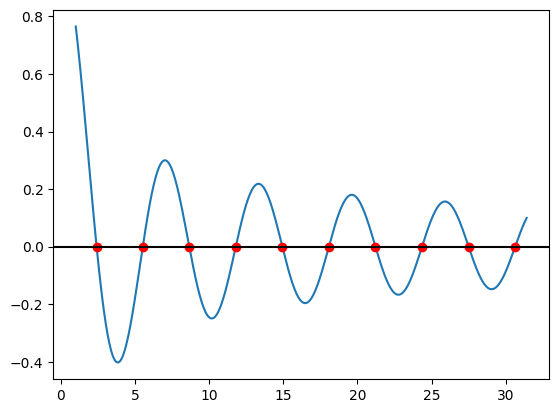
\includegraphics{Include/Images/Thesis/Documentation/NonLinear/Newtons Example 2.png}
    \caption{Newton's Method Example 2}
    \label{fig:Newton's Method Example 2}
\end{figure}